\chapter{Methods}

\section{Tracking \& Matching}
We track the predicted staff and patients across multiple frames, indicated by $t = 1 \ldots T$, by iteratively assigning the predictions, $\{ P_i^{(t)} \}_{i=1}^{M_t}$, to the latest known tracks, $\{ Q^{(t)}_{j} \}_{j=1}^{N_t}$ by greedily picking the assignment with the minimum cost:
\begin{equation}
    \argmin_{i,j} \mathcal{L}_\text{track}(P^{(t)}_i, Q^{(t-1)}_j),
\end{equation}
until either all predictions or latest tracks have been assigned exactly once. In the case of any unassigned predictions, a new track is initialized. After tracks have been assigned, the latest track $Q^{(t)}_j$ is updated with the assigned predictions. We choose the following composite loss function:
\begin{equation}
    \mathcal{L}_\text{track}(P, Q) = \alpha \norm{P_\text{3D kpts} - Q_\text{3D kpts}}{2} + \beta \norm{P_\text{class} - Q_\text{class}}{\infty},
\end{equation}
incorporating both the Euclidean distance between the 3D joint keypoints as well as the predicted person class (staff/patient), with $\alpha$ and $\beta$ weighting the influence of each term. The tracks, $T_i$, are then greedily matched to the ground truth annotations $G_j$, minimizing the loss:
\begin{equation}
    \mathcal{L}_\text{match}(T, G) = \sum_t^{T} \begin{cases}
        \norm{a^{(t)}_{\text{track}, \text{2D kpts}} - b^{(t)}_{\text{track}, \text{2D kpts}}}{2} & \text{if}\ a^{(t)}_\text{track} \in a_\text{track} \\
        \gamma & \text{otherwise}
    \end{cases}
\end{equation}
over the trajectory time horizon $t = 1,2,\ldots,T$ where $\gamma$ is the punishment for not detecting the person.

\section{Human pose sequence optimization}
% Something about using the original poses + vPoser (human pose prior) + annotated keypoints.

\section{3D scene reconstruction}


% Two approaches 

% First approach:
% First uses the relative depth disparity maps and the rendered SMPL poses in order to restore the 
% metric depth scale and offset.
% Pros:
% - Relative depth maps are often more accurate and easier for a model to learn.
% Cons:
% - The process of restoring scale and offset is not very robust and can be prone to errors if the SMPL poses don't overlap precisely with the predicted depths.  
% - The reliance of poses at different distances in order to optimally regress the scale and offset parameters.

% Second approach:
% Using metric depth estimation
% Pros:
% - Doesn't rely on rendering SMPL poses and restoring scale and offset.
% - Domain is contained to indoor hospital and carehome rooms.
% Cons:
% - Less accurate predictions


\subsection*{Restoring depth scale and offsets}
We utilize pseudo ground truth disparity maps generated by the Depth Anything model, inversely proportional to the scene depth, in order to reconstruct a point cloud of the scene. To recover the depth scale and offset we rasterize the predicted SMPL poses, extract the z-buffer, compute the inverse depth and regress the intersection with the normalized disparity maps using the Random Sample Consensus (RANSAC) algorithm robust to outliers. 

\begin{equation}
    \begin{bmatrix}p
        x \\ y \\ 1/z \\ 1
    \end{bmatrix} = \begin{bmatrix}
        f_x & 0 & 0 & p_x \\
        0 & f_y & 0 & p_y \\
        0 & 0 & 1 & 0 \\
        0 & 0 & 0 & 1
    \end{bmatrix} \begin{bmatrix}
        X \\ Y \\ Z \\ 1
    \end{bmatrix}
\end{equation}


\begin{equation}
    X = \frac{Z}{f_x} \left( x - p_x \right) , \quad Y = \frac{Z}{f_x} \left(y - p_y \right)
\end{equation}
where $f_x$, $f_y$ are the horizontal and vertical focal lenghts respectively and ($p_x$, $p_y$) is the principal point often chosen as the center $(w/2,h/2)$ of the image. 

\section{Aligning datasets}
\begin{figure}
    \centering
    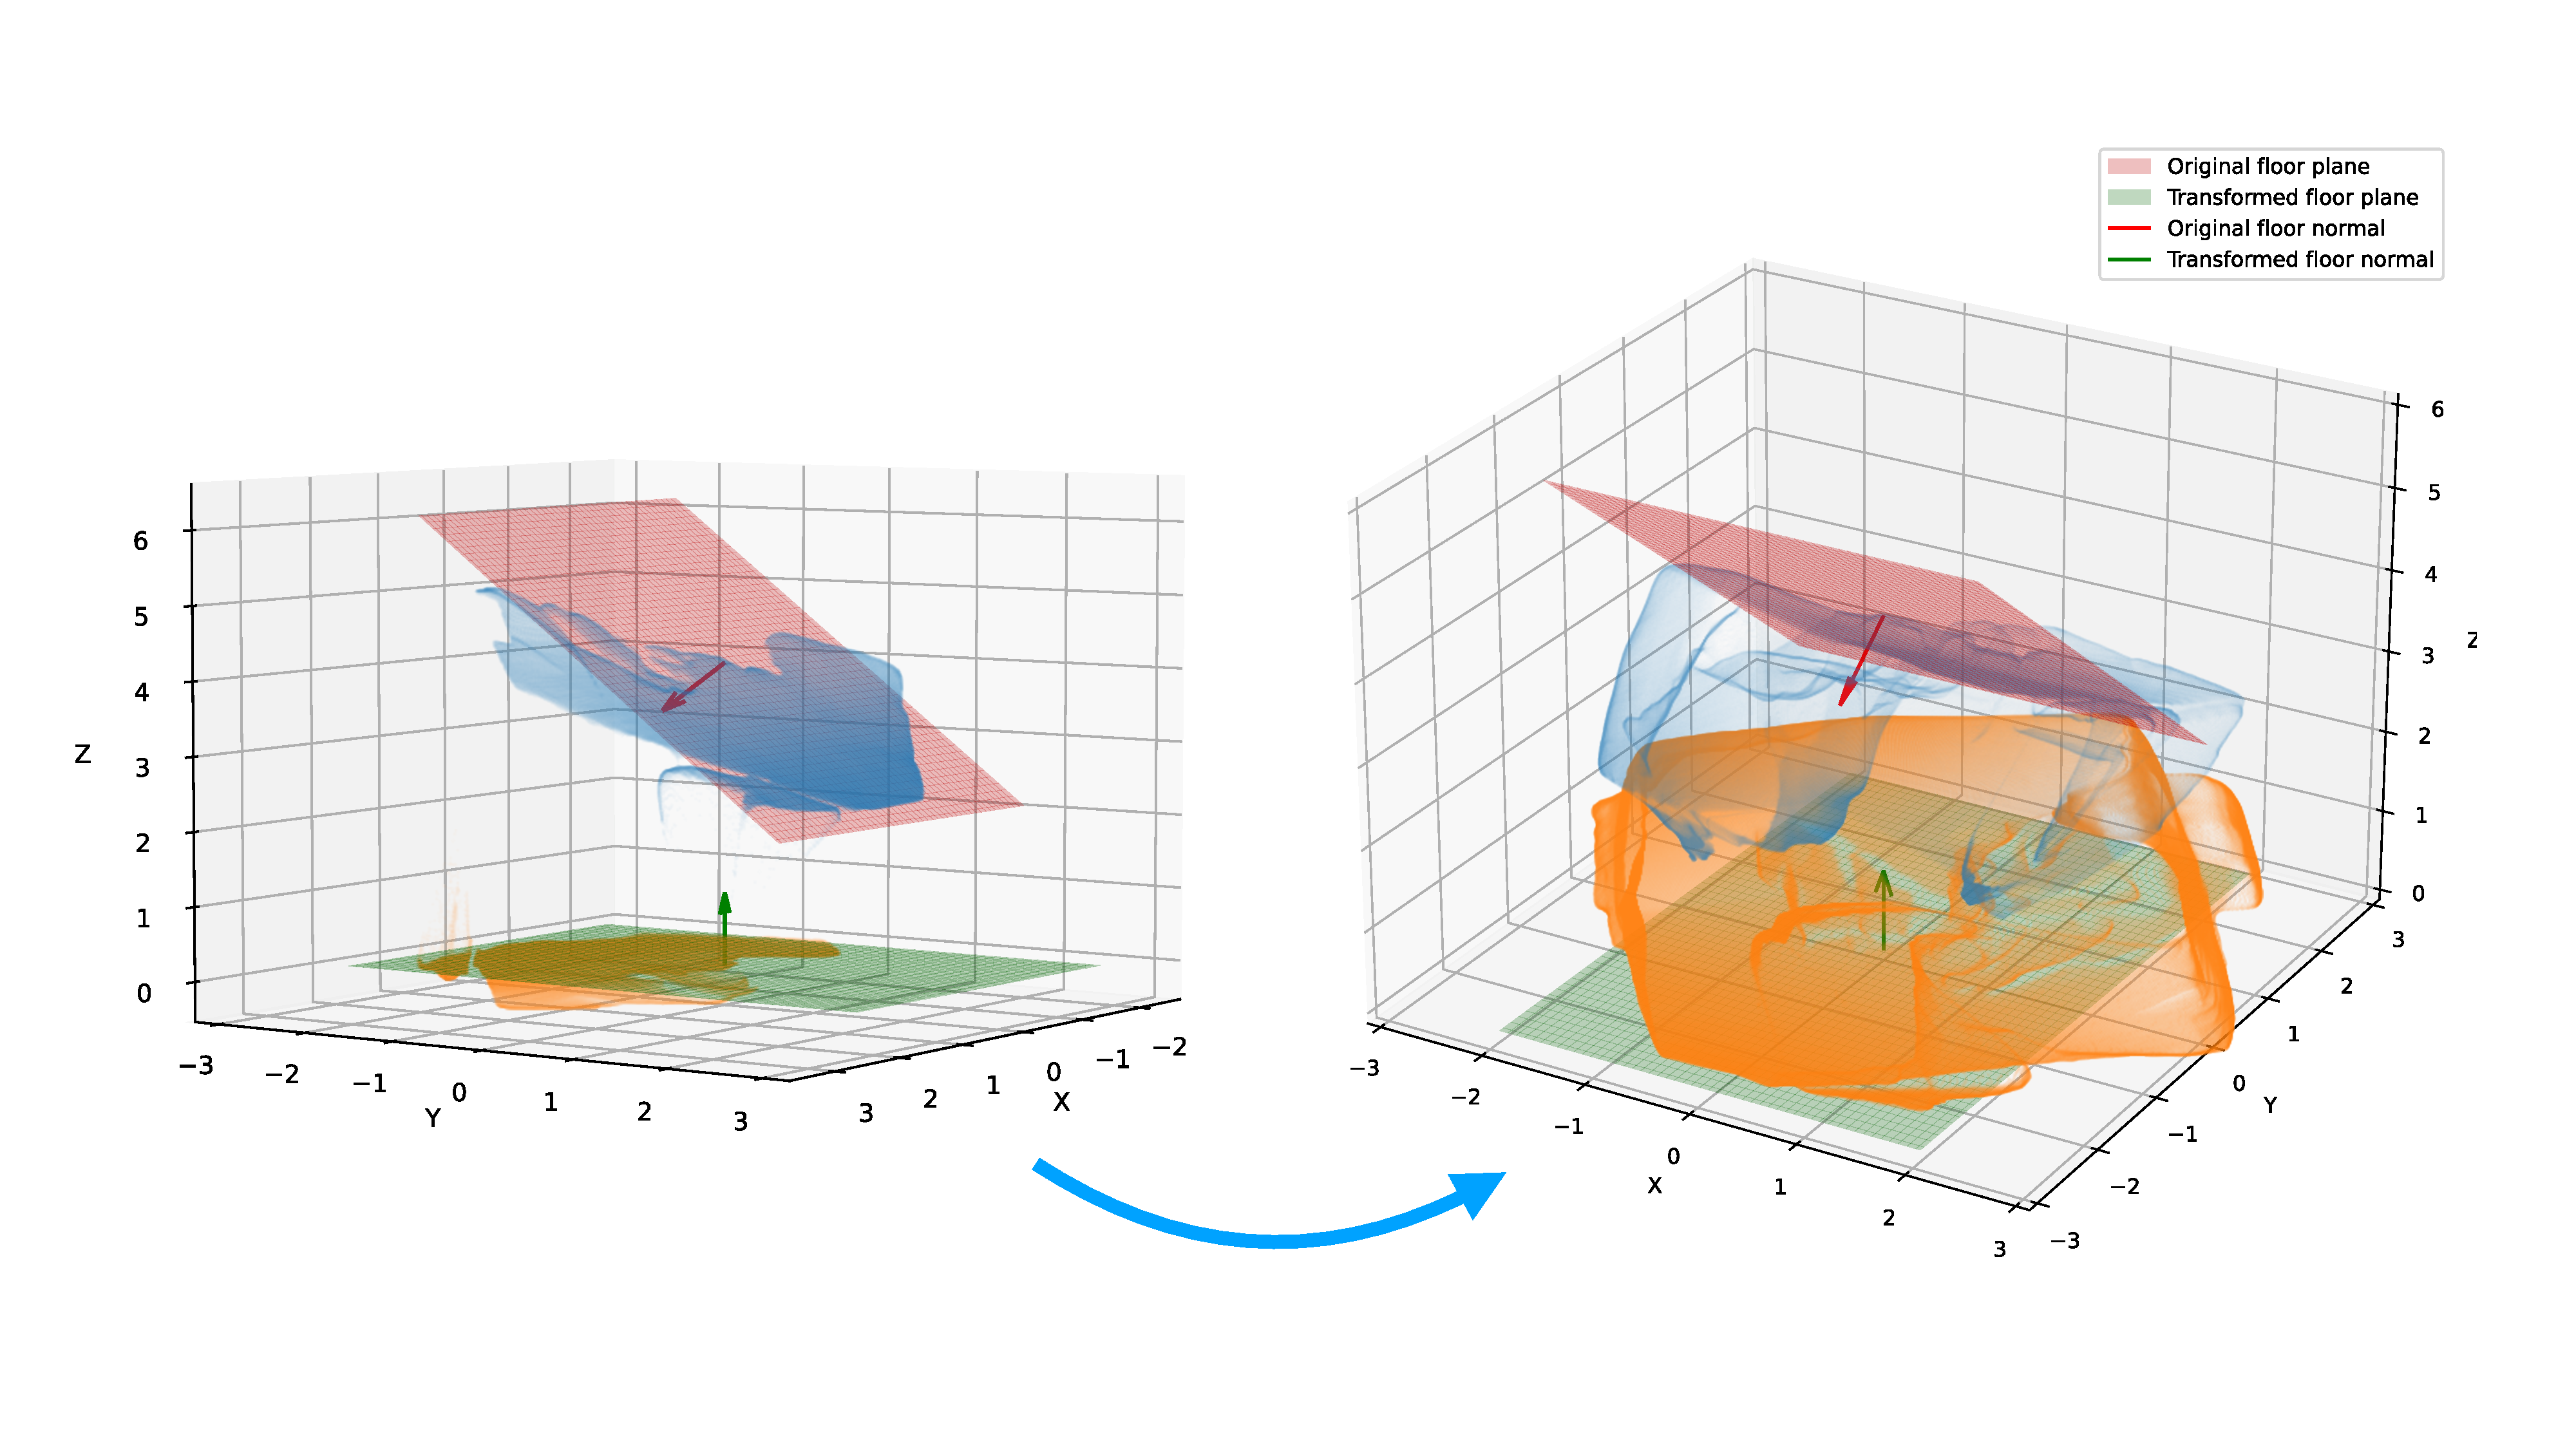
\includegraphics[width=\linewidth]{figures/rotation.pdf}
    \caption{Translation and rotation of room point cloud to align floor with XY-plane.}
    \label{fig:rotate-floor-planes}
\end{figure}

To compute the rotation matrix that aligns the normal vector $\hat{\vect{n}}_\text{floor} = \vect{n}_\text{floor} / \| \vect{n}_\text{floor} \|$ (where $\vect{n}_\text{floor} = (0, 1, \vect{b}_1)^T \times (1, 0, \vect{b}_0)^T$) of the floor plan in the camera coordinate system with the normal vector $\vect{n}_{xy} = (0, 0, 1)$ of the xy-plane, we can utilize Rodrigues' rotation formula. 

First, we construct the skew-symmetric matrix $\mathbf{K}$ from the components of the cross product vector $\vect{v} = \hat{\vect{n}}_\text{floor} \times \vect{n}_{xy}$. The skew-symmetric matrix $\mathbf{K}$ is defined as:
\begin{equation}
    \mathbf{K} = \begin{bmatrix}
        0 & -v_3 & v_2 \\
        v_3 & 0 & -v_1 \\
        -v_2 & v_1 & 0
    \end{bmatrix}
\end{equation}

Next, we compute the rotation matrix $\mathbf{R}$ using Rodrigues' rotation formula. The formula incorporates the identity matrix $\mathbf{I}$, the skew-symmetric matrix $\mathbf{K}$, and a scaling term based on the angle between the vectors. The resulting rotation matrix is given by:

\begin{equation}
    \mathbf{R} = \mathbf{I} + \mathbf{K} + \mathbf{K}^2 \left(\frac{1 - c}{s^2}\right)
\end{equation}

Here, $\mathbf{I}$ is the identity matrix, $c$ is the dot product of $\mathbf{a}$ and $\mathbf{b}$, and $s$ is the norm of the cross product vector $\mathbf{v}$. This formula ensures that the rotation matrix $\mathbf{R}$ not only aligns $\mathbf{a}$ with $\mathbf{b}$ but also preserves the orthogonality and orientation of the coordinate system.

Finally, we transform the point cloud by translating it to align the floor plane intercept with the origin, followed by rotating it using the computed rotation matrix:

\begin{equation}
    \vect{p}^* = \mathbf{R} \left(\vect{p} - (0, 0, b_0)^T \right) 
\end{equation}




\section{Motion and scene representation}
Previous work on single human motion generation uses a canonical representation 

We use a 6D continuous representation of the joint angles as according to \cite{Zhou_2019_CVPR}.
% We represent the motion similar to 


\section{Diffusion model}



